%--------------------------------------------------------------------------------------------------
% performance.tex
%
% This document define the frontespiece of the presentation
%
% author: Andrea Meneghinello
% version: 0.1
%--------------------------------------------------------------------------------------------------
\section{Performance analysis}
\begin{frame}{Performance analysis}
	UoD tested over IaaS assets by
	\begin{columns}
		\begin{column}[t]{0.33\textwidth}
			\begin{center}
				Linpack
			\end{center}
			\begin{itemize}
				\item{\tiny{CPU operations/s}}
				\item{\tiny{solve linear equations systems}}
				\item{\tiny{floating point numbers to increase complexity}}
				\item{\tiny{\url{https://goo.gl/acS2nC}}}
			\end{itemize}
		\end{column}
		\begin{column}[t]{0.33\textwidth}
			\begin{center}
				Stream
			\end{center}
			\begin{itemize}
				\item{\tiny{RAM bandwidth}}
				\item{\tiny{operations over big arrays}}
				\item{\tiny{big arrays $\rightarrow{}$ cache overflow}}
				\item{\tiny{\url{https://goo.gl/lVi2wO}}}
			\end{itemize}
		\end{column}
		\begin{column}[t]{0.33\textwidth}
			\begin{center}
				Iperf
			\end{center}
			\begin{itemize}
				\item{\tiny{network bandwidth}}
				\item{\tiny{network latency}}
				\item{\tiny{buffers transfer}}
				\item{\tiny{UoD in different physical machines}}
				\item{\tiny{\url{https://goo.gl/6aqvVE}}}
			\end{itemize}
		\end{column}
	\end{columns}
\end{frame}

\subsection{Computing benchmark}
\begin{frame}{Computing benchmark}
	\begin{columns}
		\begin{column}{0.5\textwidth}
			\begin{figure}
				\centering{}
				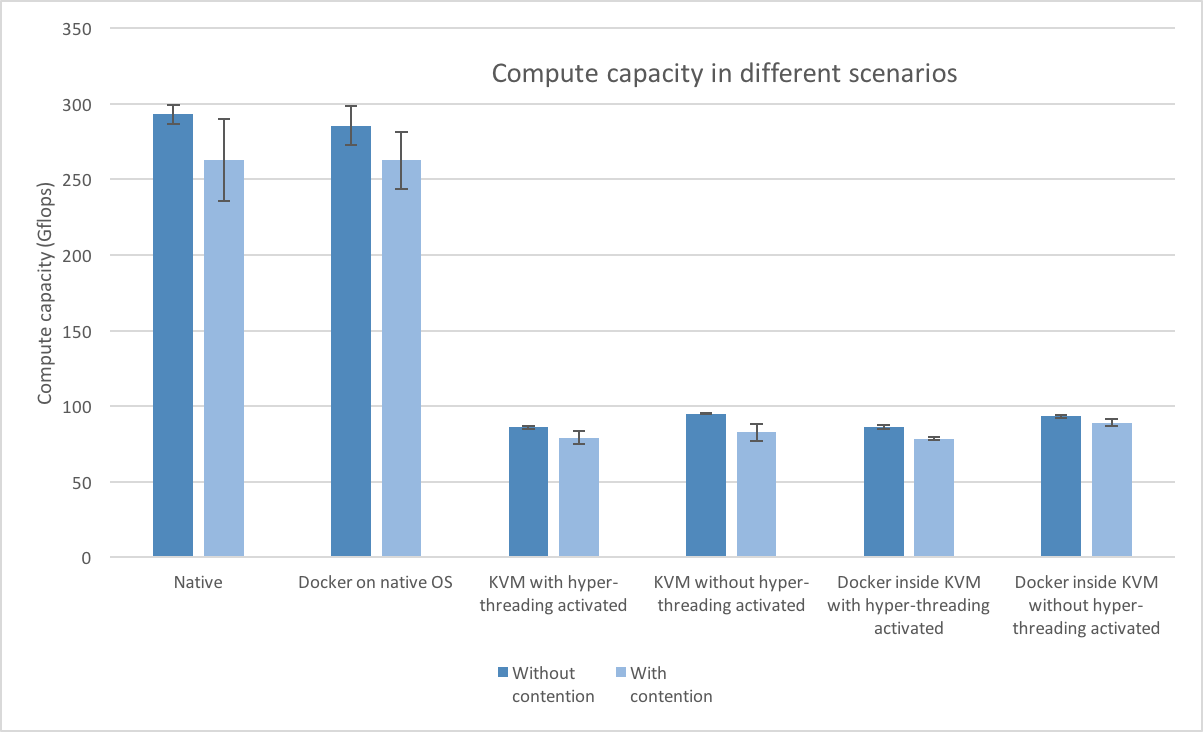
\includegraphics[scale=0.12]{images/cpu-capacity.png}
			\end{figure}
			\begin{itemize}
				\item[]{\scriptsize{A - native}}
				\item[]{\scriptsize{B - docker on native OS}}
				\item[]{\scriptsize{C - VM with hyper-threading (HP) }}
			\end{itemize}
		\end{column}
		\begin{column}{0.5\textwidth}
			\begin{figure}
				\centering{}
				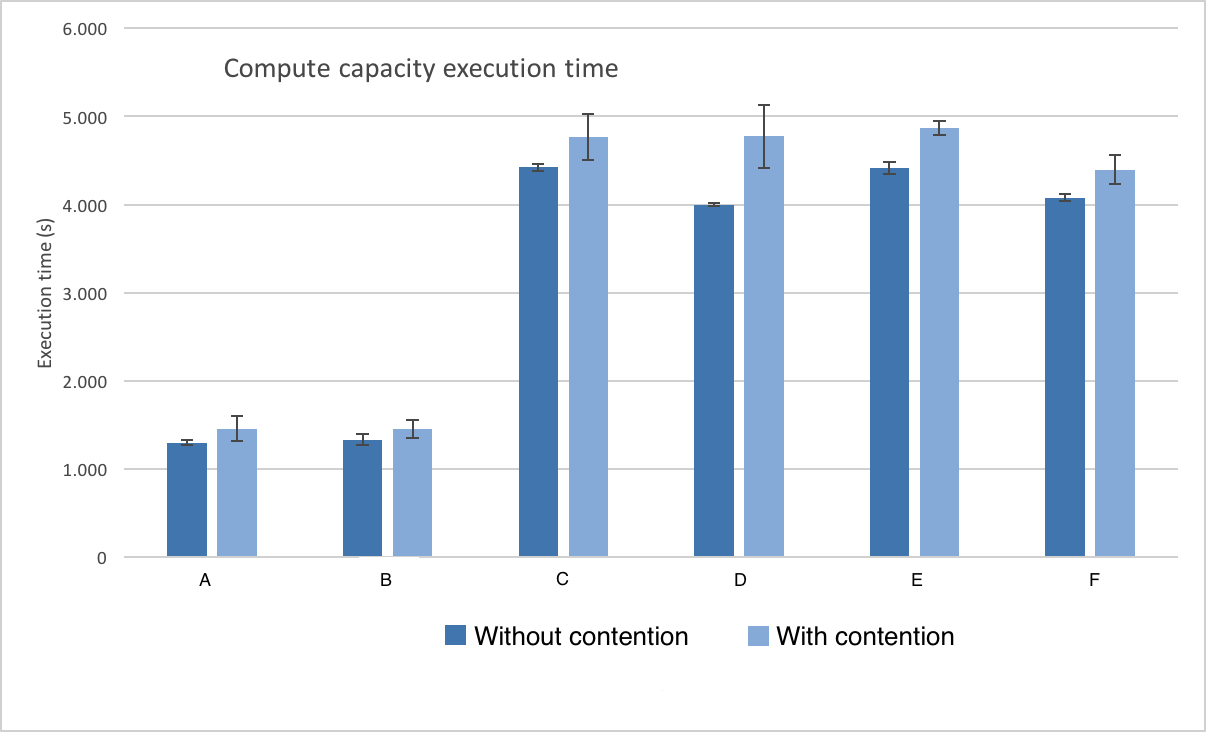
\includegraphics[scale=0.12]{images/cpu-time.png}
			\end{figure}
			\begin{itemize}
				\item[]{\scriptsize{D - VM without HP}}
				\item[]{\scriptsize{E - docker on VM with HP}}
				\item[]{\scriptsize{F - docker on VM without HP}}
			\end{itemize}
		\end{column}
	\end{columns}
\end{frame}

\subsection{Storage benchmark}
\begin{frame}{Storage benchmark}
	\begin{columns}
		\begin{column}{0.5\textwidth}
			\centering{}
			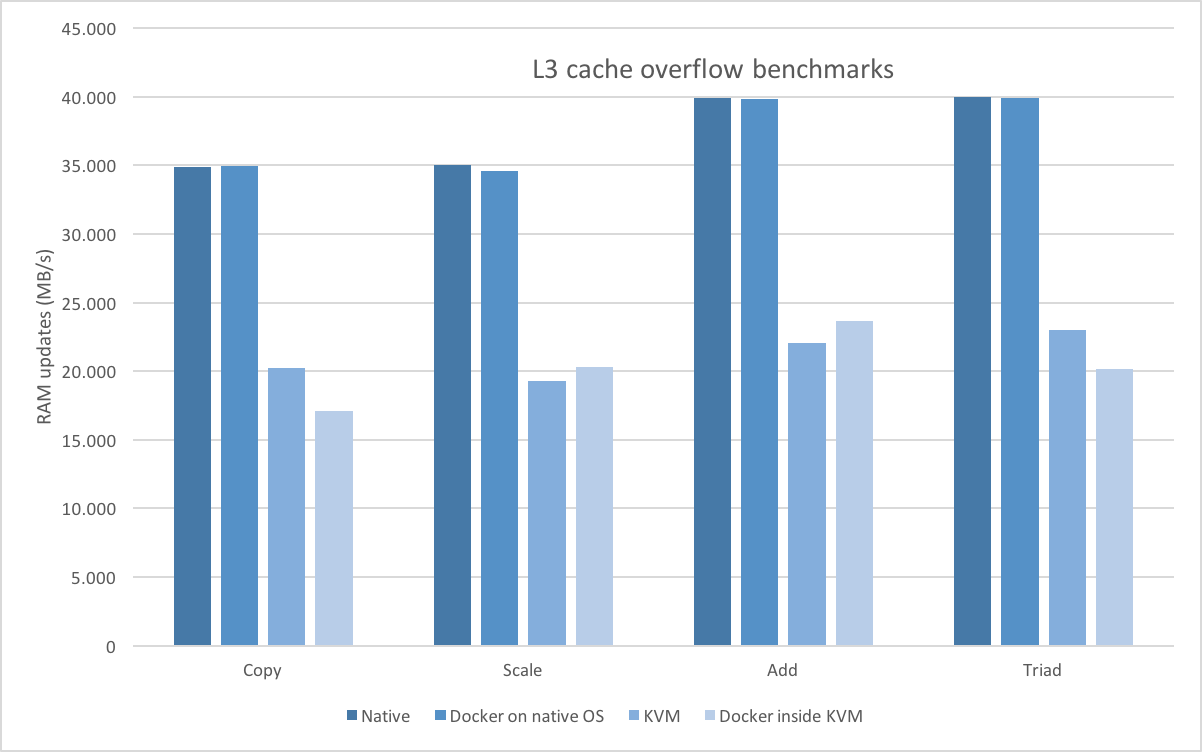
\includegraphics[scale=0.14]{images/storage-l3-capacity.png}
		\end{column}
		\begin{column}{0.5\textwidth}
			\centering{}
			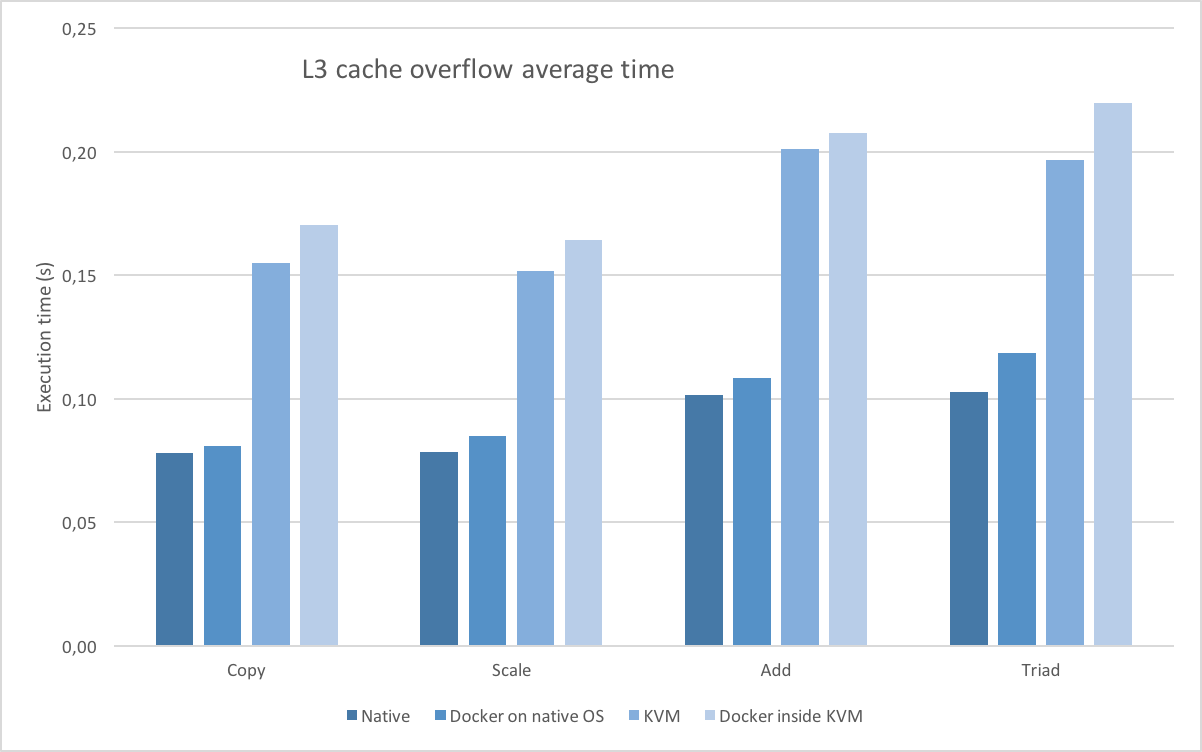
\includegraphics[scale=0.14]{images/storage-l3-time.png}
		\end{column}
	\end{columns}
\end{frame}

\subsection{Network benchmark}
\begin{frame}{Network benchmark}
	\begin{columns}
		\begin{column}{0.5\textwidth}
			\centering{}
			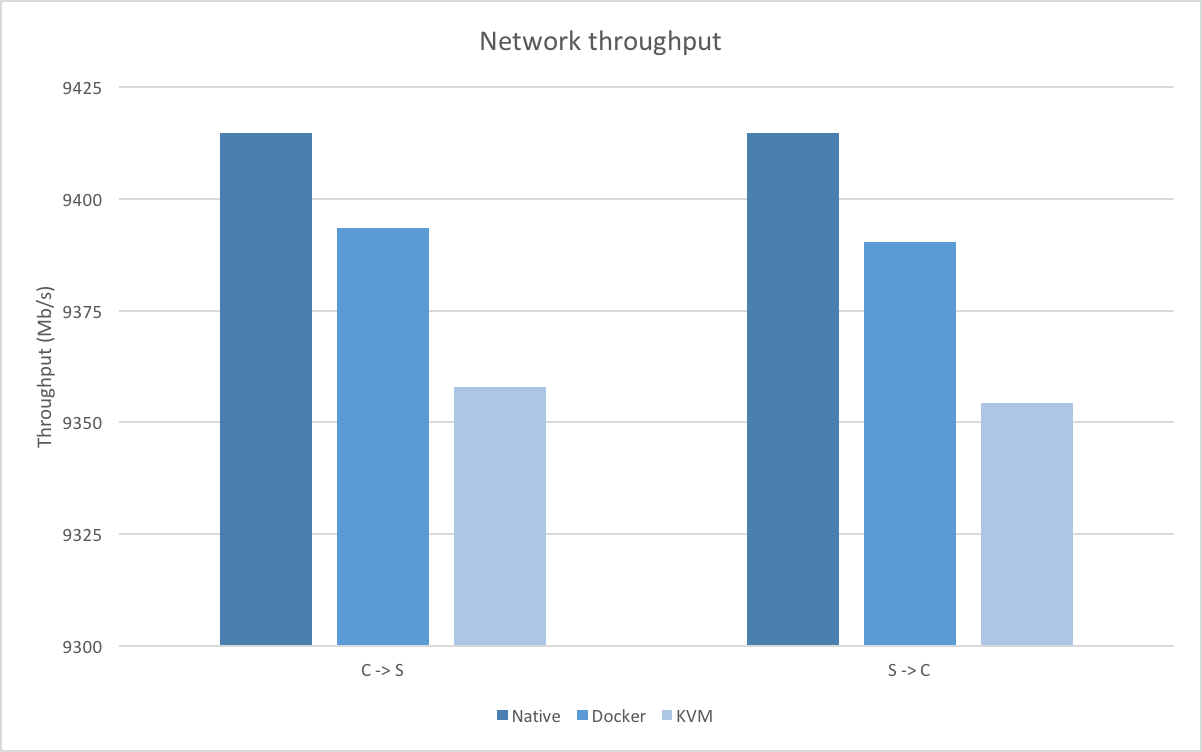
\includegraphics[scale=0.14]{images/network-throughput.png}
		\end{column}
		\begin{column}{0.5\textwidth}
			\centering{}
			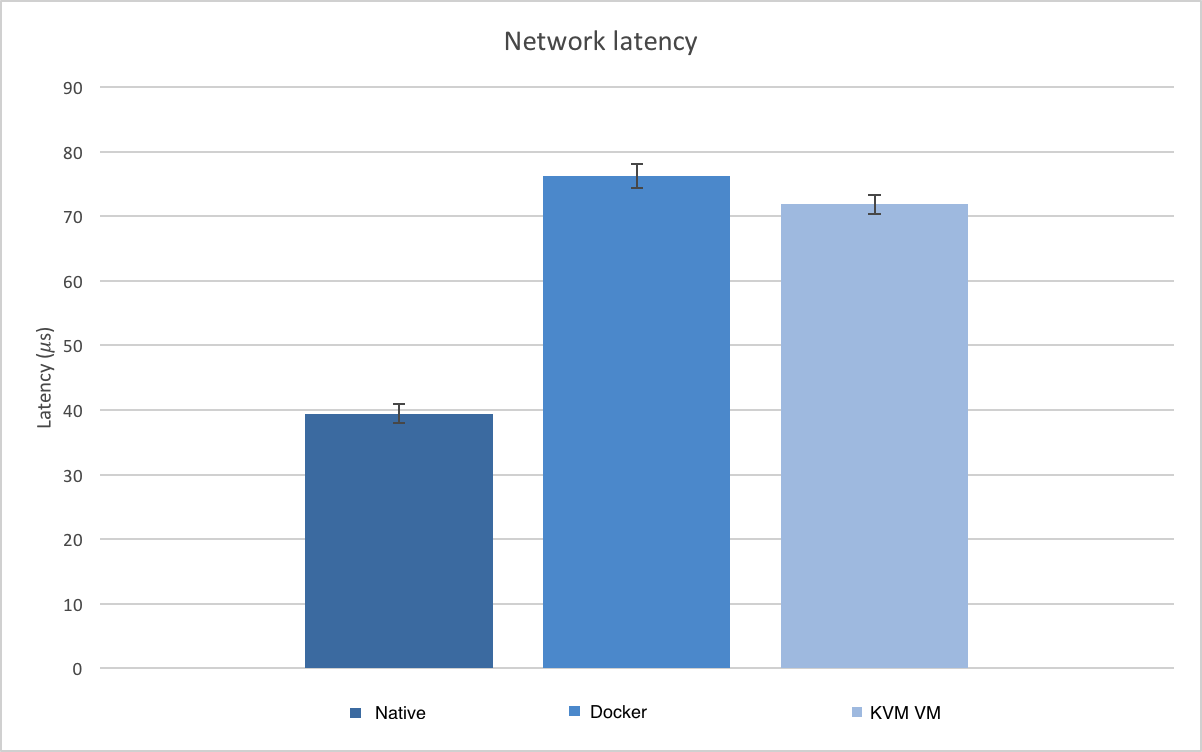
\includegraphics[scale=0.14]{images/network-latency.png}
		\end{column}
	\end{columns}
\end{frame}

\subsection{Summary}
\begin{frame}{Summary}
	\begin{columns}
		\begin{column}{0.6\textwidth}
			experiment results show
			\begin{itemize}
				\item{\footnotesize{containers make better use of IaaS assets}}
				\item{\footnotesize{containers suffer competing load}}
				\begin{itemize}
					\item{\scriptsize{high Standard Deviation}}
				\end{itemize}
				\item{\footnotesize{containers have higher network latency}}
				\begin{itemize}
					\item{\scriptsize{due to its network stack}}
				\end{itemize}
			\end{itemize}
		\end{column}
		\begin{column}{0.4\textwidth}
			\begin{figure}
				\centering{}
				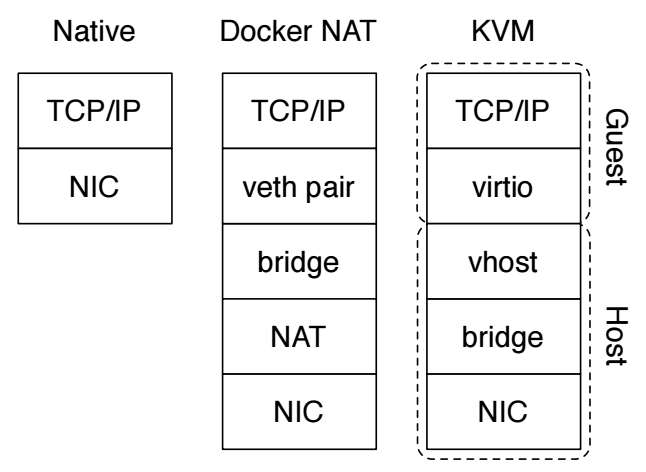
\includegraphics[scale=0.4]{images/network-stack.png}
			\end{figure}
		\end{column}
	\end{columns}
\end{frame}